\documentclass[architecture.tex]{subfiles}
\begin{document}
This chapter will give an overview of the user-centric features
that are implemented in the software. As such, it will concern the
user interface components in the frontend.
We will start off with the picture in Figure~\ref{fig:explore}, which
shows a large number of features that will be explained further.
\begin{figure}[H]
    \centering
    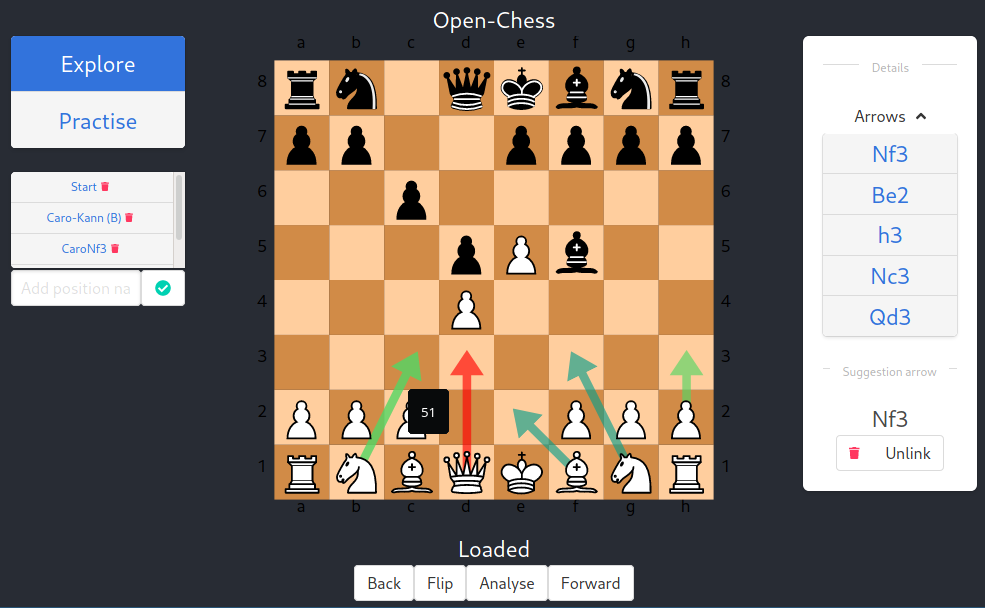
\includegraphics[width=\linewidth]{figures/explore-overview.png}
    \caption{A view of the software in a typical position}
    \label{fig:explore}
\end{figure}
We will start the discussion by a quick walk-through of the panels:
Top-left are the \textit{game modes} where the user selects between
exploring and practising (see Section~\ref{section:gamemodes}).
Below are the \textit{favorites} where the user can load a prerecorded
board position.
The right hand panel with title \textit{details} is dependent on the game mode,
here it shows a list of the arrow-indicated \textit{suggestions} with
options for the focused suggestion arrow of knight to f3.
The bottom panel holds buttons to step the game forwards and backwards,
analyse the current position, and flip the board (to see it from Black's perspective).

The following details will also give which shortkeys are available,
which simulate button presses.
\subsection{Basics}
The board is used by dragging and dropping pieces. When a piece is moved,
the move is sent to the server to be checked for validity.
On initialization, the frontend client will receive the SVG objects that
form the board, and assign mouse handlers to them.

Whenever a move has been played, either by the player or by the engine,
the user can step back (shortkey \textbf{left arrow}). When a backing has been made, the move can be
replayed by the forward-button (similarly, shortkey \textbf{right arrow}).
Whenever a new move is player, the forward-stack is emptied and
the new move is pushed to the backing stack.
The board can at any time be flipped by the bottom-panel button without
further change to the functionality. Internally, this only involves
repositioning of the SVG elements. Shortkey \textbf{f}.

The analysis button will conduct a more thorough
analysis and add new moves to the existing position.
\subsection{Favorites}
The second panel on the left-hand side are the user's \textit{favorites}.
These are positions that the user has put on the board, written a name
for in the text input field, and saved with the checkbox button.
These are meant to be used for positions that the user often is interested in.

The system will reject a name that already exists as a favorite,
as well as a position that already exists with another name.

Clicking an item in the favorite list will load the position and populating
the backing stack so that the user can load a position but still walk
backwards in the move order history.
\subsection{Game modes}
\label{section:gamemodes}
This version supports two game modes: Explore and Practise.
These are switched by clicking the top-left panels and by shortkeys
\textbf{e} and \textbf{p}, respectively.
The Explore mode is intended to try out different moves and show what
moves are recorded in the database along with their scores
(evaluations by the Stockfish engine).
The practise move will not show what the database knows about a position,
but wait for the user to make a move. It will then check the played move
against the database, and only accept moves that are good enough.
\subsubsection{Explore mode}
In Figure~\ref{fig:explore}, the game is in exploration mode. This means
that arrows of available moves are shown and color-coded by their scoring.
Green arrows indicate bght
etter moves, and blue ones are theory (as introduced
in previous chapters). The user can hover over an arrow to show its score
(seen with the move Nc3).
When an arrow is clicked, or through the list of arrows in the right-hand panel,
it is focused and can be unlinked (shortkeys \textbf{u/backspace/delete});
removed as a possible move from the board.

If a move is played that is not known (i.e. does not have an arrow),
the system will analyse it. It will then be added as a new arrow in the future.
This takes some time, the system limits the analysis to two seconds
for analyses made through playing a move in explore mode.
\subsubsection{Practise mode}
In practise mode, the arrows are not shown. After the user plays a move,
it will be checked against the list of existing moves.
If there are theory moves, the user is required to play one of them - 
otherwise the move will be rejected as inferior.
If there is no theory for the position, the user is required to have played
the known move with the highest score.

The user can request a \textit{swap} of the computer's move, prompting
it to select another of the known moves for the position.
The user may also \textit{reject} the computer's move, which performs a
swapwhile also unlinking the move so it will not be played again in the future.

Below in Figure~\ref{fig:practise} we see the same position with white to play.
Making a legal and good move, in this case any of the theory moves seen in
Figure~\ref{fig:explore}, would prompt the computer to answer with its own move.
\begin{figure}[H]
    \centering
    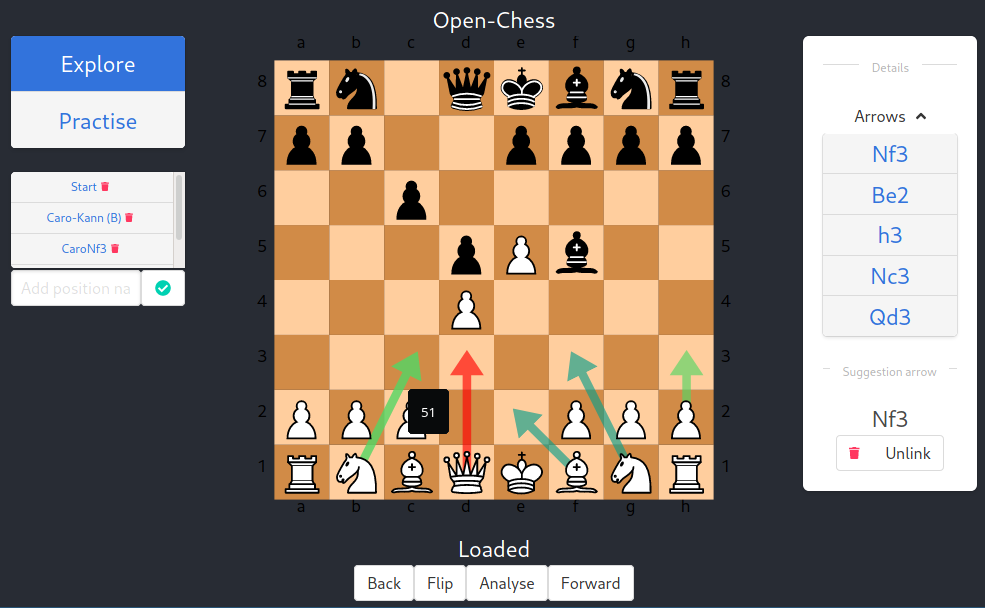
\includegraphics[width=\linewidth]{figures/explore-overview.png}
    \caption{The system in Practise mode}
    \label{fig:practise}
\end{figure}
\end{document}
